\chapter{Conceptos}\label{conceptos}

En este capítulo se presentan conceptos teóricos necesarios para la comprensión del trabajo realizado en la memoria, así como la descripción de  programas y frameworks utilizados cuyo funcionamiento y restricciones influyeron en decisiones de diseño tomadas a lo largo del desarrollo de la memoria.

\section{Definiciones}\label{definiciones}
\begin{enumerate}
\item Imagen: Una imagen se puede considerar una matriz de pixeles. El contenido de cada pixel depende del tipo de imagen, en el caso de imágenes en tonos de grises cada pixel corresponde a un valor entero entre 0 y 255, en el caso de imágenes a color cada pixel corresponde a tres números enteros cuyo significado depende del espacio de color que se utilice. En esta memoria las imágenes a color siempre corresponderán al espacio RGB, donde los tres valores del pixel corresponden a su intensidad de rojo, verde y azul respectivamente.

\item Video: Corresponde a una secuencia de imágenes (de aquí en adelante \textit{frames}) presentadas cada cierto intervalo de tiempo regular (por ejemplo 24 \textit{frames} cada segundo). 
\end{enumerate}

\section{Descriptores}\label{descriptores}
Un \emph{descriptor}~\cite{descriptors} de imagen es una forma representar dicha imagen por sus características (como su distribución de colores, orientación de bordes, textura, etc). Los descriptores son usualmente representados como vectores multidimensionales. Para compararlos es común usar una función de distancia, como por ejemplo la distancia euclideana entre vectores.

El descriptor de una imagen puede ser global o local dependiendo de si describe la imagen completa o solo sectores de ella. \\
Dado que un video es una secuencia de imágenes se puede describir usando una secuencia de descriptores de imágenes, para hacer esto típicamente se submuestrean los frames del video, es decir, aunque el video muestre 24 frames cada segundo, se pueden considerar solo algunos de ellos a intervalos regulares para describir el video. Esto funciona debido que en la mayoría de los casos dos frames consecutivos son muy similares entre sí, por lo que tomar todos los frames del video para describirlo aporta información redundante.\\
Es necesario comparar videos o imágenes utilizando descriptores en vez de comparar sus archivos bit a bit debido a que se pueden realizar transformaciones sobre una imagen que cambien totalmente los bits de su archivo sin modificar mucho el contenido de esta, como por ejemplo iluminar la imagen sumándole un valor fijo al valor de todos sus pixeles.

\section{Detección de copia basada en contenido}\label{copias}

La detección de copia basada en contenido o \emph{Content Based Copy Detection} (CBCD) se define como~\cite{tesis}: \\
Sea $V$ una colección de documentos multimedia (imágenes, audio, video) y sea $q$ un documento de búsqueda. Una \emph{detección de copia basada en contenido} consiste en encontrar y recuperar todos los documentos $v \in V$ de la colección tales que $q$ ``es una copia'' de $v$.

En el contexto de esta memoria los documentos corresponden a videos, y la relación ``es una copia'' se refiere a que el video de consulta corresponde a una grabación del video original.

Para establecer si dos videos cumplen la relación de copia es necesario tener una manera de comparar su contenido. Es muy probable que la grabación no sea idéntica al video original debido a transformaciones de color y perspectiva inherentes a la grabación, sin embargo es posible comparar los videos por las \textit{características} presentes en ellos, como sus colores, formas, etc. Esta comparación de características se realiza por medio de \emph{descriptores}.

La Figura~\ref{deteccion_copia} ilustra las etapas del proceso de detección de copia. El primer paso, correspondiente a la Figura~\ref{detect_extract}, es extraer descriptores del video de consulta y de cada uno de los videos de la colección de referencia (estos últimos pueden ser precalculados y utilizados en múltiples consultas). El siguiente paso, ilustrado en la figura~\ref{detect_search}, es realizar una \emph{búsqueda por similitud}, que corresponde a identificar por cada descriptor del video de consulta, los descriptores más \emph{similares} entre los de la colección de referencia. En este contexto los descriptores \emph{más similares} corresponden a los que presenten menor distancia en el espacio vectorial. Finalmente se toma la información de descriptores más similares y se buscan secuencias crecientes de descriptores que correspondan al mismo video. Se razona que si para cada descriptor del video de consulta, se encuentra entre sus más cercanos a descriptores de un mismo video, entonces el video de consulta representa una copia de un segmento del video de la colección de referencia.

\begin{figure}
\centering
\subcaptionbox{Extracción de descriptores. Con mayúscula se representan los videos y con mínuscula y subíndice sus descriptores\label{detect_extract}}{%
  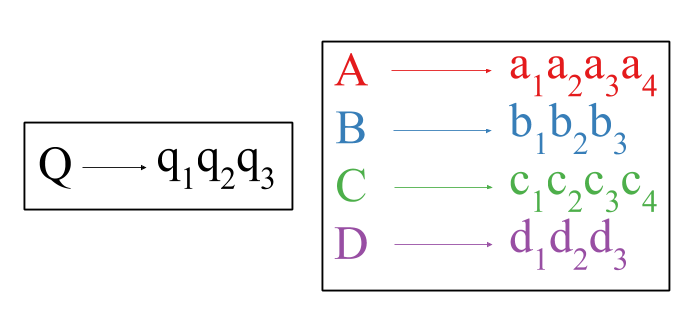
\includegraphics[width=0.6\textwidth]{imagenes/cap2/descriptor_extraction.png}%
  }\par\medskip
\subcaptionbox{Búsqueda por similitud y detección\label{detect_search}}{%
  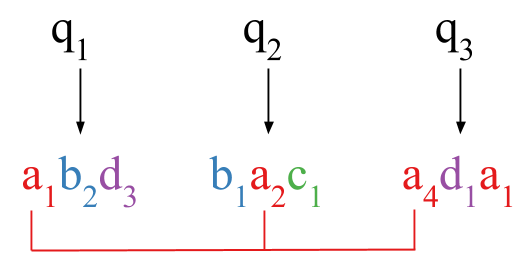
\includegraphics[width=0.6\textwidth]{imagenes/cap2/similarity_search.png}%
  }
\caption{Etapas del proceso de detección de copias en video.}
\label{deteccion_copia}
\end{figure}

\section{Android}\label{android}
Android es un sistema operativo desarrollado por Google~\cite{android}, es principalmente usado en dispositivos móviles como smartphones y tablets. Las aplicaciones para Android son programas escritos en el lenguaje de programación Java que hacen uso de las bibliotecas del \emph{Software Development Kit} (SDK) de Android para realizar llamadas al sistema operativo. Esta sección presenta brevemente conceptos del sistema Android necesarios para entender la implementación del trabajo realizado.

\subsection*{Actividades y Fragmentos}

Una actividad corresponde a cualquier clase que extienda de la clase Activity\footnote{\url{http://developer.android.com/guide/components/activities.html}} o alguno de sus descendientes, asimismo un fragmento corresponde a clases que extiendan de Fragment\footnote{\url{http://developer.android.com/guide/components/fragments.html}}. Las actividades y fragmentos controlan elementos de la interfaz gráfica de la aplicación. La vista de la interfaz gráfica es definida usando XML para especificar los elementos de la interfaz y sus posiciones. El comportamiento en cambio se controla desde actividades y fragmentos, que asignan métodos \emph{listener} a los distintos elementos de la interfaz. 
En general se usa una actividad para manejar un proceso dentro de la aplicación y varios fragmentos se encargan cada uno de una etapa del proceso.

\subsection*{Comunicación entre aplicaciones}

Existen ciertos procesos que pueden ser necesarios para diversos tipos de aplicaciones, como por ejemplo mostrar los archivos de una carpeta para que el usuario elija uno, o reproducir un archivo de video. Si bien es posible que cada aplicación implemente su propia solución a estos problemas un dispositivo Android usualmente cuenta con aplicaciones predefinidas que realizan estos procesos. Cuando una aplicación requiere tales procesos puede realizar una llamada al sistema que invoque una aplicación predefinida y, una vez se obtenga un resultado (se seleccionó un archivo, se reprodujo el video, etc) se le entregan los resultados de vuelta a la aplicación original. Esta llamada se realiza a través de un objeto \emph{Intent}\footnote{\url{http://developer.android.com/reference/android/content/Intent.html}}, que representa una descripción abstracta del trabajo que se quiere realizar. Android provee una lista de intents estándar para acciones comunes. 
El siguiente código muestra como se puede invocar la aplicación por defecto de la cámara para grabar un video y guardarlo a archivo:
\begin{lstlisting}[style=JavaInputStyle]
    Intent intent = new Intent(MediaStore.ACTION_VIDEO_CAPTURE);
    videoFile = getOutputFile();
    intent.putExtra(MediaStore.EXTRA_OUTPUT, videoFile);
    intent.putExtra(MediaStore.EXTRA_DURATION_LIMIT, 5);

    startActivityForResult(intent, CAPTURE_VIDEO_ACTIVITY_REQUEST_CODE);
\end{lstlisting}


En la primera línea se selecciona el intent apropiado. Es posible agregarle opciones dependiendo de la acción requerida, en el ejemplo se especifica el archivo de salida y la duración máxima del video. Finalmente se invoca la aplicación usando el método \texttt{startActivityForResult} que recibe al intent y un código que identifica a la aplicación original. Para obtener el resultado de la acción basta implementar el método \texttt{onActivityResult} que será llamado automáticamente por el sistema.  

\section{Procesamiento de imágenes en Android}\label{img_proc}

Los dispositivos móviles disponen de limitada memoria y capacidad de computo en comparación con un computador de escritorio. Es por esto que para implementar la extracción de descriptores en Android fue necesario buscar alternativas que permitieran hacer uso eficiente de los recursos disponibles, después de investigar se encontraron dos opciones prometedoras. Por un lado está la librería OpenCV\footnote{\url{http://opencv.org/}} de procesamiento de imágenes y visión por computador. Esta librería es ampliamenta usada en la industria y se encuentra disponible para multiples plataformas, incluido el sistema Android. Está implementada en C/C++ y cuenta con interfaces para Java y Python. Se utilizó un libro escrito por los autores de la librería como apoyo para la implementación~\cite{opencv}. Por otro lado Android cuenta con un framework propio para aplicaciones que requieran alta capacidad de computo llamado RenderScript\footnote{\url{http://developer.android.com/guide/topics/renderscript/compute.html}}.

Antes de comenzar la implementación de la memoria se pusieron a prueba ambas alternativas. Se implementaron dos operaciones típicas de procesamiento de imágenes, convertir una imágen de color a gris y realizar una convolución, además se implementó unos de los descriptores usados en la memoria. Se implementaron de manera que fueran capaces de recibir \emph{frames} de la cámara del dispositivo mientras esta realiza una grabación. Se midió la cantidad de tiempo requerido por cada implementación para realizar cada operación, además se usaron dos calidades de video distintas para medir el efecto del aumento en el tamaño de la imagen. Los resultados de estas pruebas se resumen en la Figura~\ref{renderscript_vs_opencv}, podemos ver que en todos los casos la implementación en Renderscript resultó ser más rápida que la de OpenCV. Dados estos resultados se decidió utilizar el framework RenderScript para implementar las tareas de procesamiento de imágenes en el dispositivo móvil. 
    \begin{figure}[!h]
		\centering
		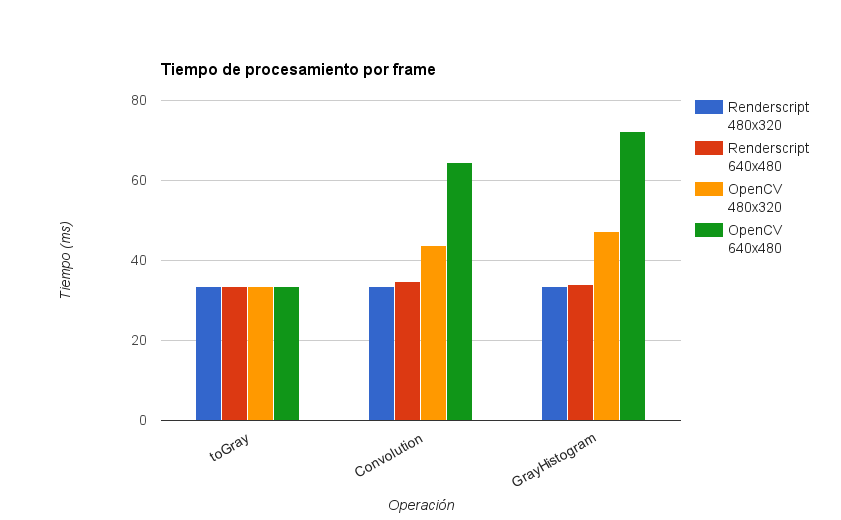
\includegraphics[scale=0.5]{imagenes/cap2/renderscript_vs_opencv.png}
		\caption{Resultados de la comparación entre RenderScript y OpenCV.}
		\label{renderscript_vs_opencv}
	\end{figure}

En la siguiente sección se detalla el funcionamiento del framework RenderScript.

%%%%%%%%%%%% RENDERSCRIPT %%%%%%%%%%%%%%%%%%%%%%%%%
\section{RenderScript}\label{renderscript}
RenderScript es un framework de Android diseñado para lograr alto rendimiento al correr código en paralelo, aunque algoritmos secuenciales también pueden verse beneficiados por él. El funcionamiento de RenderScript se basa en escribir un \emph{kernel} de procesamiento que el sistema puede distribuir a los procesadores disponibles en el dispositivo, como los múltiples núcleos de la CPU, o la GPU. 
Los kernel se escriben en un lenguaje derivado de C99, a continuación se presenta un ejemplo de un kernel que convierte una imagen en RGBA a escala de grises.

\begin{lstlisting}[style=CInputStyle]
#pragma version(1)
#pragma rs java_package_name(fquintan.renderscripttest)
#pragma rs_fp_relaxed

void  rgba_to_grayscale(uchar4 *v_in, uchar *v_out,
                                uint32_t x, uint32_t y) {
    uchar red = (*v_in).r;
    uchar green = (*v_in).g;
    uchar blue = (*v_in).b;
    uchar intensity = (uchar) 0.2989*red + 0.5870*green + 0.1140*blue;
    *v_out = intensity;
}
\end{lstlisting}

Las primeras tres líneas corresponden a configuración de Renderscript. La función \texttt{\justify rgb\_to-\_grayscale} recibe 4 parámetros. El primero es un puntero a un \texttt{uchar4}, un tipo nativo de RenderScript que representa un pixel con cuatro elementos, este corresponde a un pixel de la imagen de entrada. El segundo es un puntero a un \texttt{uchar} que corresponde a un pixel de la imágen de salida. El tercer y cuarto parámetro corresponden a las coordenadas que ocupan los pixeles de entrada y salida en sus respectivas imágenes. El cuerpo de la función extrae los valores de rojo, verde y azul del pixel de entrada, calcula el valor de gris correspondiente y lo asigna al pixel de salida.

El código anterior se ejecutará una vez para cada pixel de la imagen de entrada, creando así la imagen de salida. El sistema operativo distribuirá esta ejecución de la mejor manera posible haciendo uso de los múltiples núcleos de la CPU o GPU para poder realizar el cálculo de varios pixeles en paralelo.

El caso anterior es simple dado que todos los pixeles son independientes entre sí, por lo que no requiere esfuerzo del programador sincronizar su ejecución. Para casos más complejos RenderScript cuenta con primitivas de sincronización que permiten tener acceso exclusivo a una variable compartida para modificar su valor.

Suponiendo que el código anterior se guarda en el archivo \texttt{RGBA2Gray.rs} al compilar se generará la clase Java
\texttt{ScriptC\_RGBA2Gray} con código que permite ejecutar el script. Para ejecutar primero debemos pasar el input a un formato que RenderScript pueda recibir, para esto el framework provee la clase \texttt{Allocation}\footnote{\url{http://developer.android.com/reference/android/renderscript/Allocation.html}}. Una Allocation es un contenedor para los elementos de entrada y salida de un script. Para el ejemplo anterior debemos crear dos Allocations como sigue:

\begin{lstlisting}[style=JavaInputStyle]
Allocation inAllocation;
Allocation outAllocation;

rs = RenderScript.create(context);

Type.Builder inType = new Type.Builder(rs, Element.U8_4(rs));
inType.setX(imageWidth);
inType.setY(imageHeight);

inAllocation = Allocation.createTyped(rs, inType.create(),
            Allocation.USAGE_SCRIPT);

Type.Builder outType = new Type.Builder(rs, Element.U8(rs));
outType.setX(imageWidth);
outType.setY(imageHeight);

outAllocation = Allocation.createTyped(rs, outType.create(),
            Allocation.USAGE_SCRIPT);
\end{lstlisting}

Notemos que en las líneas 8 y 13 se define el tipo de elemento de cada Allocation, en este caso, la entrada corresponde a pixeles de tipo \texttt{uchar\_4}, que se traducen en Java al tipo \texttt{Element.U8\_4}, mientras que la salida contenía pixeles de tipo \texttt{uchar}, que se traducen al tipo \texttt{Element.U8}. El tamaño de las Allocation debe ser definido al momento de crearlas, en este caso ambas Allocations tienen el mismo tamaño, pero RenderScript permite definir Allocations de entrada y salida de distintos tamaños.

Finalmente hay que poblar de datos la Allocation de entrada, correr el script y extraer los datos de la Allocation de salida como muestra el siguiente código:

\begin{lstlisting}[style=JavaInputStyle]
Bitmap imageRGBA;
Bitmap imageGray;
// ... inicializar los bitmaps
inAllocation.copyFrom(imageRGBA);
ScriptC_RGBA2Gray script = new ScriptC_RGBA2Gray(rs);
script.forEach(inAllocation, outAllocation);
outAllocation.copyTo(imageGray);
\end{lstlisting}

La clase Allocation cuenta con métodos \texttt{copyFrom} para poblar Allocations a partir de múltiples estructuras de datos como Bitmaps o arreglos numéricos, por otro lado se cuenta con métodos \texttt{copyTo} para extraer los resultados de la Allocation de salida. El método \texttt{forEach} de la clase \texttt{ScriptC\_RGBA2Gray} ejecuta el script sobre las Allocations recibidas.

Se utilizó el framework RenderScript para implementar el cálculo de descriptores en el dispositivo móvil, los detalles de esta implementación se discuten en el capítulo 4 de este informe.

%%%%%%%%%%%% PVCD %%%%%%%%%%%%%%%%%%%%%%%%%
\section{P-VCD}\label{pvcd}
%Por qué?
P-VCD es un software de detección de copias en video \cite{p-vcd1}, es decir, detecta segmentos de video similares dentro de una colección. Fue implementado como parte de una tesis de doctorado y fue probado participando en la competencia de Content-based copy detection de TRECVID en 2010 y 2011 \cite{p-vcd2}.

P-VCD logra detectar videos similares siguiendo el siguiente algoritmo:
\begin{enumerate}
\item Calcular descriptores para una base de datos de videos. El programa cuenta con múltiples tipos de descriptores tanto locales como globales que pueden ser utilizados. Se guardan en distintos archivos tanto los descriptores como la información de que frame representa cada descriptor.
\item Dado un video de consulta se calculan y guardan sus descriptores.
\item Para cada descriptor del video de consulta se encuentran en la base de datos sus vecinos más cercanos, esto es, los descriptores que tengan menor distancia al descriptor de consulta según una función de distancia apropiada, como lo es por ejemplo la distancia euclideana entre vectores.
\item Usando los vecinos más cercanos encontrados, se usa la información de a que frame y a que video corresponden para identificar secuencias donde los vecinos más cercanos correspondan a una secuencia creciente de frames del mismo video. Si se encuentra tal secuencia se guarda información del video original y de la ubicación de la secuencia de frames. Pueden encontrarse múltiples posibles copias para una mismo video de consulta, así como se puede no encontrar ningún candidato a copia. 
\end{enumerate}

El programa está construido de manera modular de forma que cada etapa del proceso de búsqueda se puede realizar independiente de las otras, esto hace que P-VCD sea útil para el desarrollo de esta memoria, pues se puede crear e indexar una base de datos de videos de forma offline, para luego saltarse la etapa de extracción de descriptores del objeto de búsqueda, entregándole al sistema los descriptores calculados por otro programa y formateados de la misma manera y prosiguiendo a la etapa de detección de copias.

P-VCD se invoca usando comandos de consola para cada etapa del proceso de búsqueda. A continuación se detallan los comandos necesarios para realizar la extracción de descriptores y la búsqueda de videos similares.

Suponiendo que todos los videos que se utilizarán como referencia están ubicados en el directorio \texttt{videos\_dir}, se procede a inicializar una base de datos con el comando:
\begin{lstlisting}[style=BashInputStyle]
    > pvcd_db -new -db database videos_dir
\end{lstlisting}

Este comando crea el directorio \texttt{database} que contiene el archivo \texttt{files.txt}, este archivo contiene información de todos los videos encontrados en \texttt{videos\_dir}, como sus dimensiones, tipo de archivo, cantidad de frames, etc. De ahora en adelante para trabajar con los videos basta referenciar la base de datos \texttt{database}. El paso siguiente es calcular una segmentación con el comando:
\begin{lstlisting}[style=BashInputStyle]
    > pvcd_db -segment -db database -seg SEGCTE_0.25
\end{lstlisting}
La segmentación define el conjunto de frames que se usará para describir cada video, en el ejemplo anterior se extraen frames a intervalos regulares de 0.25 segundos. Como resultado de este comando se crea el directorio \texttt{segmentations} dentro de \texttt{database}, que contiene un archivo de texto con extensión .seg por cada video de la base de datos. Cada línea del archivo .seg contiene el momento exacto al cual corresponde el frame extraído dentro del video original.
El siguiente paso es calcular los descriptores, para esto se usa el comando:
\begin{lstlisting}[style=BashInputStyle]
    > pvcd_db -extract -db database -seg SEGCTE_0.25 -desc [DESCRIPTOR] -alias [ALIAS]
\end{lstlisting}

Este comando utiliza la segmentación creada anteriormente para calcular descriptores a cada frame seleccionado, el parámetro \texttt{[DESCRIPTOR]} corresponde a la definición de alguno de los descriptores disponibles en P-VCD, mientras que \texttt{[ALIAS]} corresponde a un parámetro opcional que puede usarse para renombrar un descriptor, de ahora en adelante se puede referir al descriptor usando su alias. Como resultado del comando anterior se crea un directorio \texttt{descriptors} dentro de \texttt{database}, que contiene un archivo binario de extensión .bin para cada video de la base de datos. Cada archivo .bin contiene todos los descriptores calculados para el video correspondiente. Con esto ya tenemos calculados los descriptores de la base de datos.\\

Para iniciar una búsqueda el primer paso es repetir los pasos anteriores para el video de consulta, con los comandos:
\begin{lstlisting}[style=BashInputStyle]
    > pvcd_db -new -db database video_de_consulta.mp4
    > pvcd_db -segment -db consulta -seg SEGCTE_0.25
    > pvcd_db -extract -db consulta -seg SEGCTE_0.25 -desc [DESCRIPTOR] -alias [ALIAS]
\end{lstlisting}
Cabe destacar que el tipo de descriptor y el alias deben ser iguales a los usados anteriormente para poder realizar la búsqueda. El siguiente paso es crear un perfil del búsqueda
\begin{lstlisting}[style=BashInputStyle]
    > pvcd_search -new -profile perfil -query consulta
        -reference database -desc [ALIAS] -distance L2
\end{lstlisting}
Este ejemplo crea un nuevo perfil de consulta, que usará la base de datos ubicada en \texttt{database} como referencia y la ubicada en \texttt{consulta} como objeto de consulta, se usará el descriptor renombrado como \texttt{[ALIAS]} para la búsqueda y la distancia \texttt{L2} (distancia euclideana) como función de distancia. Seguido esto podemos ejecutar la búsqueda de vecinos más cercanos para cada descriptor:
\begin{lstlisting}[style=BashInputStyle]
    > pvcd_search -ss -profile perfil -knn 3
\end{lstlisting}
Este comando ejecuta la búsqueda, encontrando para cada descriptor de la base de datos de consulta, sus tres vecinos más cercanos. Los resultados se guardan por defecto en el archivo de texto \texttt{ss,segments-knn\_3.txt} del directorio \texttt{perfil}. El paso final es encontrar secuencias entre los vecinos más cercanos usando el comando:
\begin{lstlisting}[style=BashInputStyle]
    > pvcd_detect -detect -ss "perfil\ss,segments-knn\_3.txt"
        -minLength 1s -out "perfil\detections.txt"
\end{lstlisting}
Con este comando se puede especificar el archivo que contiene los vecinos más cercanos, así como un archivo de salida donde se escribirá la información de los candidatos a copia detectados. También se puede especificar con el parámetro \texttt{minLength} mínimo largo que debe tener una secuencia de frames del mismo video para ser considerado un candidato a copia. Después de ejecutar esta serie de comandos el archivo \texttt{detections.txt} contendrá los candidatos a copia.

De la descripción anterior podemos ver que el proceso de búsqueda de P-VCD está separado en etapas autocontenidas, cualquiera de las cuales puede ser fácilmente reemplazada por otro programa que obtenga los mismos resultados, siempre y cuando se respete el formato de los archivos de entrada y salida de cada etapa. Esto fue especialmente útil para el desarrollo de la memoria, pues permitió realizar el cálculo de descriptores del video de consulta de forma independiente, integrando los resultados de este cálculo con las siguientes etapas de la búsqueda sin mayores problemas. 
